\documentclass[a4paper,11pt]{article}
\usepackage{graphicx}
\usepackage{enumerate}

\begin{document}

\begin{flushright}

\vspace{1.1cm}

{\bf\Huge Problem Set 5}

\rule{0.25\linewidth}{0.5pt}

\vspace{0.5cm}
%Put Authors
Justin Ely
\linebreak
\newline
%Put Author's affiliations
\footnotesize{605.411 Foundations of Computer Architecture \\}
\vspace{0.5cm}
% Date here below
04 October, 2016
\end{flushright}

\noindent\rule{\linewidth}{1.0pt}

%%%%%%%%%%%%%%%%%%%%%%%%%%%%%%%%%%%%%%%%%%%%%%%%%%%%%%%%%%

\section*{1)}

%%%%%%%%%%%%%%%%%%%%%%%%%%%%%%%%%%%%%%%%%%%%%%%%%%%%%%%%%%

\section*{2)} 
\begin{itemize}
 \item r-type
 \item load word
 \item branch (since it does a subtract)?
\end{itemize}

%%%%%%%%%%%%%%%%%%%%%%%%%%%%%%%%%%%%%%%%%%%%%%%%%%%%%%%%%%

\section*{3)}
\begin{tabular}{| c | c | c | c | c | }
  \hline	
       A & B & X  & Min-term & Max-term \\  \hline
       0 & 0 & 1 & A`B` & \\  \hline
       1 & 0 & 0 & & A` + B\\  \hline
       0 & 1 & 0 & & A + B`\\  \hline
       1 & 1 & 1 & AB & \\  \hline
\end{tabular} \\

\begin{figure}[h]
\caption{PLA.}
\centering
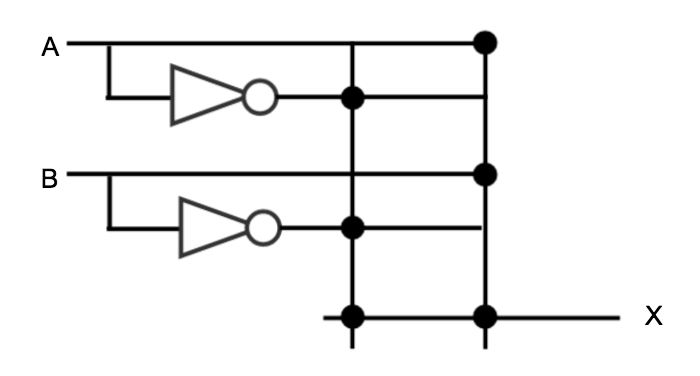
\includegraphics[width=.8\textwidth]{problem_3_pla.png}
\end{figure}


%%%%%%%%%%%%%%%%%%%%%%%%%%%%%%%%%%%%%%%%%%%%%%%%%%%%%%%%%%

\section*{4a)}
\begin{tabular}{| c | c | c | c |}
  \hline	
   000100 & 00000 & 00100 & 0000000000001010 \\  \hline
\end{tabular} \\

The op-code says this is a BEQ instruction.  This goes through states 0, 1, 8 on the state diagram.

\section*{4b)}
0, 1, 2, 6, 8

\section*{4c)}


\section*{4d)}


\section*{4e)}
The branch is comparing register \$0 to register \$4.  Since \$0 = \$4 = 0, the branch is taken.  


%%%%%%%%%%%%%%%%%%%%%%%%%%%%%%%%%%%%%%%%%%%%%%%%%%%%%%%%%%

\section*{5)}
\begin{tabular}{| c | c | c | c | c | c | c | c | c | }
  \hline	
       X2 & X1 & X0  & a & b & c & d & minterm & maxterm \\  \hline
       0 & 0 & 0  &  &  & y &   & X2`X1`X0` & X2 + X1 + X0 \\  \hline
       1 & 0 & 0  &  & y &  & y & X2X1`X0` & X2` + X1 + X0  \\  \hline
       0 & 1 & 0  &  & y & y &   & X2`X1X0` & X2 + X1` + X0 \\  \hline
       1 & 1 & 0  & y &  &  &  y & X2X1X0` & X2` + X1` + X0 \\  \hline
       0 & 0 & 1  &  & y & y &   & X2`X1`X0 & X2 + X1 + X0` \\  \hline
       1 & 0 & 1  & y &  &  &  y & X2X1`X0 & X2` + X1 + X0` \\  \hline
       0 & 1 & 1  & y &  & y &   & X2`X1X0 & X2 + X1` + X0` \\  \hline
       1 & 1 & 1  &  &  &  &  y & X2X1X0 & X2` + X1` + X0` \\  \hline
\end{tabular} \\

\section*{5a)}
X = (X2X1X0') + (X2X1`X0) + (X2`X1X0)

\section*{5b)}
X = (X2X1`X0`) + (X2`X1X0`) + (X2`X1`X0)

\section*{5c)}
X = (X2`X1`X0`) + (X2`X1X0`) + (X2`X1`X0) + (X2`X1X0)

\section*{5d)}
X = (X2X1`X0`) + (X2X1X0`) + (X2X1`X0) + (X2X1X0)

%%%%%%%%%%%%%%%%%%%%%%%%%%%%%%%%%%%%%%%%%%%%%%%%%%%%%%%%%%

\section*{6)}



%%%%%%%%%%%%%%%%%%%%%%%%%%%%%%%%%%%%%%%%%%%%%%%%%%%%%%%%%%

\section*{7)}
From the state diagram given in the lectures:\\

\begin{itemize}
  \item beq: 3
  \item j: 3
  \item or: 4
  \item add: 4 
  \item lw: 5
  \item sw: 4
  \item bne: 3
\end{itemize}


%%%%%%%%%%%%%%%%%%%%%%%%%%%%%%%%%%%%%%%%%%%%%%%%%%%%%%%%%%

\section*{8)}
\begin{itemize}
  \item lw \$2,40(\$4):  Uses the memory system when it is retrieving the specified word, the ALU to calculate the address, and the register file to see in which register to write the loaded word.
  \item add \$3,\$6,\$7: Uses the ALU do perform the arithmetic, and the register file to read operands and write result.
  \item slt \$5,\$6,\$7:  Uses the ALU to check if one register is less than another, and the register file to read operands and set the result.
  \item sw \$6,44(\$4):  Uses the register file and ALU to retrieve and calculate the address in memory to put the register value.
  \item and \$9,\$11,\$10:  Uses the ALU to perform the AND operation, and the register file to read operands and write result.
  \item or \$21,\$27,\$8: USes the ALU to perform the OR operation, and the register file to read operands and write result.
\end{itemize}

%%%%%%%%%%%%%%%%%%%%%%%%%%%%%%%%%%%%%%%%%%%%%%%%%%%%%%%%%%

\end{document}
